% !TEX program = xelatex
% 计算物理 第二次作业报告
\RequirePackage{expl3}
\ExplSyntaxOn
\msg_redirect_name:nnn { fontspec } { no-script } { info }
\ExplSyntaxOff
\documentclass[UTF8,a4paper,12pt]{ctexart}

\usepackage{amsmath,amssymb}
\usepackage{graphicx}
\usepackage{geometry}
\usepackage{listings}
\usepackage{xcolor}
\usepackage{float}
\usepackage{fancyhdr}
\usepackage{hyperref}

\geometry{margin=2.5cm}
\graphicspath{{imgs/}}
\hypersetup{colorlinks=true,linkcolor=blue,urlcolor=blue}

% 页码居中置于页面底部
\pagestyle{fancy}
\fancyhf{}
\fancyfoot[C]{\thepage}
\renewcommand{\headrulewidth}{0pt}
\renewcommand{\footrulewidth}{0pt}

% 章节序号用中文：一、 二、 （一）（二）
% aftername 控制序号与标题文字之间的间距，置空以缩短间隔
\ctexset{
  section/number       = \chinese{section},
  section/name         = {,、},
  section/aftername    = {},
  subsection/number    = \chinese{subsection},
  subsection/name      = {（,）},
  subsection/aftername = {},
}

\lstset{
  basicstyle=\ttfamily\small,
  breaklines=true,
  frame=single,
  numbers=left,
  numberstyle=\tiny\color{gray},
  keywordstyle=\color{blue!70!black},
  commentstyle=\color{green!45!black},
  stringstyle=\color{red!60!black},
  showstringspaces=false,
  columns=flexible,
  language=Python,
}

\title{第二次作业——$\alpha$ 粒子源的能量标定\\与未知粒子能量的反演}
\author{课程名称：计算物理\quad 授课教师：靳亚康\\[0.2em]专业：应用物理\quad 姓名：刘越\quad 学号：2024120101019}
\date{\today}

\begin{document}
\maketitle

% =====================================================================
\section{题目解析}

\subsection{题目背景}

$\alpha$ 粒子源放出的是\textbf{单能}粒子：核素发生 $\alpha$ 衰变时，粒子能量由母核与子核的能级差决定，是一个确定的数值，在核数据表中有精确记载。这样的粒子射入探测器并把全部能量沉积在其中，探测器就输出一个电脉冲；在探测器与电子学系统工作于线性区的条件下，\textbf{脉冲幅度 $S$ 与沉积能量 $E$ 成正比}。

于是产生了一个实用的物理问题：先用若干个\textbf{能量已知}的标准 $\alpha$ 源测出对应的 $(E_i,S_i)$，建立“能量—幅度”的映射；再把某个\textbf{能量未知}的粒子打进来，只测得它的脉冲幅度，就可以反过来推出它的能量。这一过程称为探测器的\textbf{能量标定}，由幅度反推能量则称为\textbf{逆回归}。

本题给出了 5 组标定数据（见 \texttt{data\_HW.txt}，能量跨度 $5156\sim5805$ keV），并要求求出信号幅度 $S_0=1502$ mV 的未知粒子的能量。

\subsection{任务拆解}

题目的三条要求为：

\begin{enumerate}
  \item 从所提供的文件读取数据，自行选择计算方法（推荐拟合）；
  \item 编写 Python 程序实现该计算；
  \item 绘图并讨论。
\end{enumerate}

第 1 条与上次作业不同：数据不再写在程序里，而是放在独立的数据文件中，需要先做\textbf{文件解析}。第 2、3 条则要求给出完整的结果、图形与讨论。

\subsection{方法选择}

标定的核心是确定 $S$ 与 $E$ 的关系。取一次式 $S=aE+b$，其中斜率 $a$（mV/keV）反映探测器与电子学系统的\textbf{能量-幅度转换系数}，截距 $b$（mV）是\textbf{电子学零点偏移}。选一次式有两条理由：探测器在线性区工作时输出幅度正比于沉积能量，这是物理预期；而且 5 个点只覆盖 $649$ keV（约为数据重心的 $12\%$），在这么窄的窗口内任何光滑的非线性响应都可以用一次式很好地逼近。

需要反解 $E$ 时有两个方向可走，本题两种都做，互相校核：

\begin{itemize}
  \item \textbf{正向拟合}：以 $E$ 为自变量拟合 $S=aE+b$，再代数反解 $E_0=(S_0-b)/a$；
  \item \textbf{反向拟合}：以 $S$ 为自变量直接拟合 $E=pS+q$，代入即得 $E_0=pS_0+q$。
\end{itemize}

此外再做一次\textbf{线性插值}（只取 $S_0$ 相邻的两点），作为不依赖拟合的参照。这三种做法都属于“拟合/插值”，实现简单，也足以回答题目所问。

% =====================================================================
\section{算法}

\subsection{数据读取}

数据文件共两行，以制表符分隔，每行的第一个字段是名称标签，其后才是数据。读取时按行切分、跳过首字段并转为浮点数组：

\begin{lstlisting}
with open(path, encoding='utf-8') as f:
    lines = [ln.strip() for ln in f if ln.strip()]
# the 1st field of each row is a label, the rest are numbers
E = np.array([float(v) for v in lines[0].split('\t')[1:]], dtype=float)
S = np.array([float(v) for v in lines[1].split('\t')[1:]], dtype=float)
\end{lstlisting}

读得 $\mathbf{E}=[5156,5440,5486,5763,5805]$ keV，$\mathbf{S}=[1390,1455,1561,1640,1705]$ mV，共 $n=5$ 组。

\subsection{正向拟合与反演}

最小化残差平方和 $\sum_i\big(S_i-aE_i-b\big)^2$，得

\begin{equation}
  a=\frac{S_{xy}}{S_{xx}},\qquad b=\bar S-a\bar E ,
\qquad
  S_{xy}=\sum_i(E_i-\bar E)(S_i-\bar S),\quad
  S_{xx}=\sum_i(E_i-\bar E)^2 ,
\end{equation}

拟合质量用\textbf{残差标准差} $s=\sqrt{\frac{1}{n-2}\sum_i r_i^2}$（$r_i=S_i-aE_i-b$）衡量，斜率与截距的标准误为

\begin{equation}
  \sigma_a=\frac{s}{\sqrt{S_{xx}}},\qquad
  \sigma_b=s\sqrt{\frac1n+\frac{\bar E^2}{S_{xx}}} .
\end{equation}

反解 $E_0=(S_0-b)/a$ 时，$a$、$b$ 都带误差，一阶误差传递给出

\begin{equation}
  \sigma_{E_0}=\frac{s}{|a|}\sqrt{\,1+\frac1n+\frac{(S_0-\bar S)^2}{a^2S_{xx}}\,},
\end{equation}

其中 $1$ 表示 $S_0$ 作为一次单次实测值本身带有 $s$ 大小的散布；$\frac1n$ 来自标定直线高度（响应均值 $\bar S$）的不确定；最后一项则是斜率 $\hat a$ 的误差被 $S_0$ 偏离数据重心的杠杆所放大。

\subsection{反向拟合}

把 $S$ 当自变量拟合 $E=pS+q$，形式与上面完全对称，只需把 $E$ 与 $S$ 互换：

\begin{equation}
  p=\frac{S_{xy}}{S_{ss}},\qquad q=\bar E-p\bar S ,\qquad
  S_{ss}=\sum_i(S_i-\bar S)^2 ,
\end{equation}

残差标准差记为 $s_E=\sqrt{\frac{1}{n-2}\sum_i(E_i-pS_i-q)^2}$（单位 keV），于是

\begin{equation}
  E_0=pS_0+q,\qquad
  \sigma_{E_0}=s_E\sqrt{1+\frac1n+\frac{(S_0-\bar S)^2}{S_{ss}}} .
\end{equation}

\subsection{线性插值}

取 $S_0$ 所夹的两个标定点 $(S_1,E_1)$、$(S_2,E_2)$，直接线性插值：

\begin{equation}
  E_0=E_1+(E_2-E_1)\cdot\frac{S_0-S_1}{S_2-S_1}.
\end{equation}

\subsection{核心代码}

三种方法的实现（对应 \texttt{hw2\_t1.py} 节选）：

\begin{lstlisting}[caption={三种计算方法（hw2\_t1.py 节选）}]
# --- 1) forward fit  S = a*E + b, then invert ---
a, b   = np.polyfit(E, S, 1)
s      = np.sqrt(np.sum((S - (a*E + b))**2) / (n - 2))   # residual std
Sxx    = np.sum((E - E.mean())**2)
E0_fwd = (S0 - b) / a
u_fwd  = (s/abs(a)) * np.sqrt(1 + 1/n + (S0 - S.mean())**2 / (a**2 * Sxx))

# --- 2) reverse fit  E = p*S + q ---
p, q   = np.polyfit(S, E, 1)
s_E    = np.sqrt(np.sum((E - (p*S + q))**2) / (n - 2))
Sss    = np.sum((S - S.mean())**2)
E0_rev = p*S0 + q
u_rev  = s_E * np.sqrt(1 + 1/n + (S0 - S.mean())**2 / Sss)

# --- 3) linear interpolation between the two neighbours of S0 ---
lo     = np.searchsorted(S, S0) - 1
E0_int = np.interp(S0, S[lo:lo+2], E[lo:lo+2])
\end{lstlisting}

% =====================================================================
\section{结果讨论}

\subsection{拟合结果}

程序读入 5 组数据后，正向拟合得到

\begin{equation}
  \boxed{\;S=(0.469938\pm0.077740)\,E-(1048.56\pm430.30)\;}
\qquad(\text{mV},\;\text{keV})
\end{equation}

其中相关系数 $r=0.9613$，$R^2=0.9241$，残差标准差 $s=41.12$ mV，最大残差 $52.91$ mV。反向拟合得到 $E=(1.966494\pm0.325310)\,S+(2481.54\pm505.70)$ keV。各点的拟合值与残差列于表 \ref{tab:points}，图 \ref{fig:fit} 为数据点、拟合直线与反演结果的合图。

\begin{table}[H]
  \centering
  \caption{标定数据、正向拟合值与残差（$S_{\text{fit}}=aE+b$）}
  \label{tab:points}
  \begin{tabular}{|c|c|c|c|c|}
    \hline
    $i$ & $E_i$ (keV) & $S_i$ (mV) & $S_{\text{fit}}$ (mV) & 残差 $r_i$ (mV) \\
    \hline
    1 & 5156 & 1390 & 1374.44 & $+15.56$ \\
    \hline
    2 & 5440 & 1455 & 1507.91 & $-52.91$ \\
    \hline
    3 & 5486 & 1561 & 1529.52 & $+31.48$ \\
    \hline
    4 & 5763 & 1640 & 1659.70 & $-19.70$ \\
    \hline
    5 & 5805 & 1705 & 1679.43 & $+25.57$ \\
    \hline
  \end{tabular}
\end{table}

\begin{figure}[H]
  \centering
  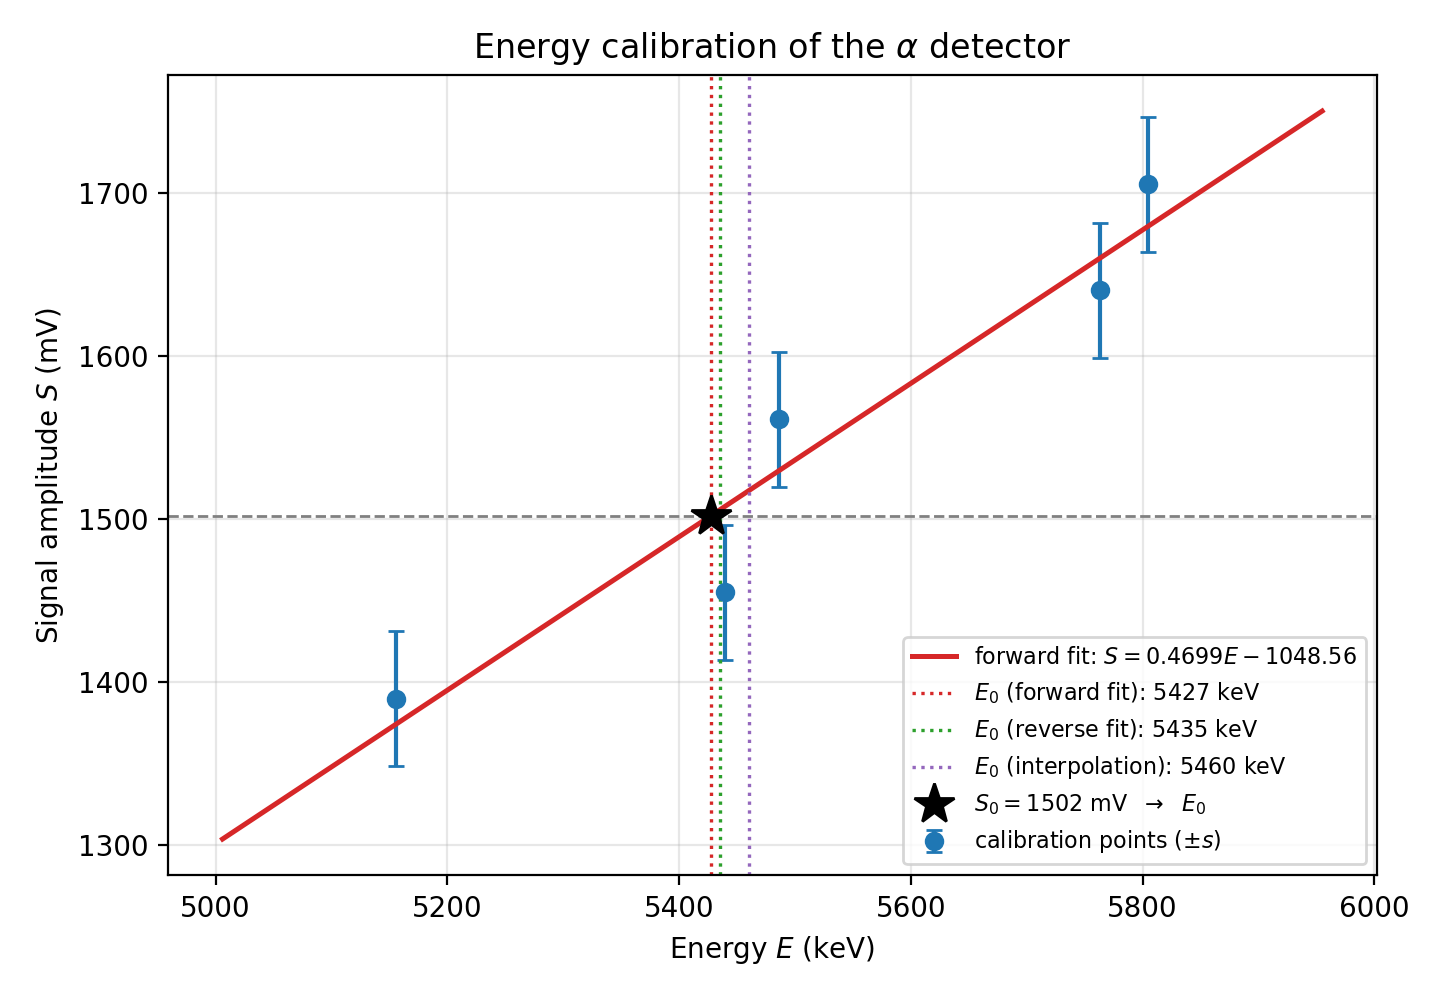
\includegraphics[width=0.72\textwidth]{hw2_fit.png}
  \caption{标定直线、5 个标定点（误差棒为残差标准差 $s$）与 $S_0=1502$ mV 对应的反演结果。}
  \label{fig:fit}
\end{figure}

有一点值得注意：正向拟合的斜率 $a=0.4699$ mV/keV，其倒数 $1/a=2.128$ keV/mV，而反向拟合的斜率 $p=1.966$ keV/mV，两者相差约 $7.6\%$。这不是算错，而是回归方向不同带来的\textbf{衰减效应}——以含误差的 $S$ 作自变量时，拟合出的斜率会系统偏小。两者的乘积恰好等于决定系数：

\begin{equation}
  a\cdot p=0.469938\times1.966494=0.9241=R^2 ,
\end{equation}

而几何平均 $\sqrt{a\cdot p}=0.9613$ 正好等于相关系数 $r$。这说明两种方向的拟合是自洽的，其差异有明确的统计来源，因此两者都保留、互为校核，而不必强行取舍。

\subsection{待测粒子的能量}

把 $S_0=1502$ mV 代入三种方法，结果列于表 \ref{tab:methods}。

\begin{table}[H]
  \centering
  \caption{三种方法得到的 $S_0=1502$ mV 对应的能量}
  \label{tab:methods}
  \begin{tabular}{|p{3.4cm}|p{6.4cm}|c|}
    \hline
    方法 & 说明 & $E_0$ (keV) \\
    \hline
    正向拟合逆回归 & $E_0=(S_0-b)/a$，并以 $E$ 为精确自变量 & $5427.4$ \\
    \hline
    反向拟合 & $E_0=pS_0+q$，直接由 $S_0$ 计算 & $5435.2$ \\
    \hline
    线性插值 & 只取 $S_0$ 相邻两点 $(1455,1561)$ mV & $5460.4$ \\
    \hline
  \end{tabular}
\end{table}

三种方法的结果最大只相差 $32.96$ keV，远小于正向拟合给出的 $1\sigma=97.35$ keV（相对 $1.79\%$），说明\textbf{结果对方法选择不敏感}——不论用正向拟合、反向拟合还是插值，答案都落在同一个范围内。以正向拟合为准（标定的全部误差都落在 $S$ 上，$E$ 是精确自变量，这样处理在统计上最合适），取

\begin{equation}
  \boxed{\;E_0=(5427\pm97)\ \text{keV}\approx5.43\ \text{MeV}\;}
\end{equation}

即\textbf{待测粒子的能量约为 5.43 MeV}。反向拟合与插值给出的 $5435$、$5460$ keV 与之相差不到 $1\sigma$，可作为交叉印证。

\subsection{残差检验}

图 \ref{fig:resid} 是正向拟合的残差图。5 个残差依次为 $+15.56$、$-52.91$、$+31.48$、$-19.70$、$+25.57$ mV，符号交错，全部落在 $\pm1.3\,s$ 之内，既没有连续同号的长串，也没有“中间低两头高”的系统弯曲。若真实响应是弯曲的，残差会呈现可辨认的趋势；现在的交错分布正是随机噪声的表现，说明\textbf{用一条直线标定是合适的}。

\begin{figure}[H]
  \centering
  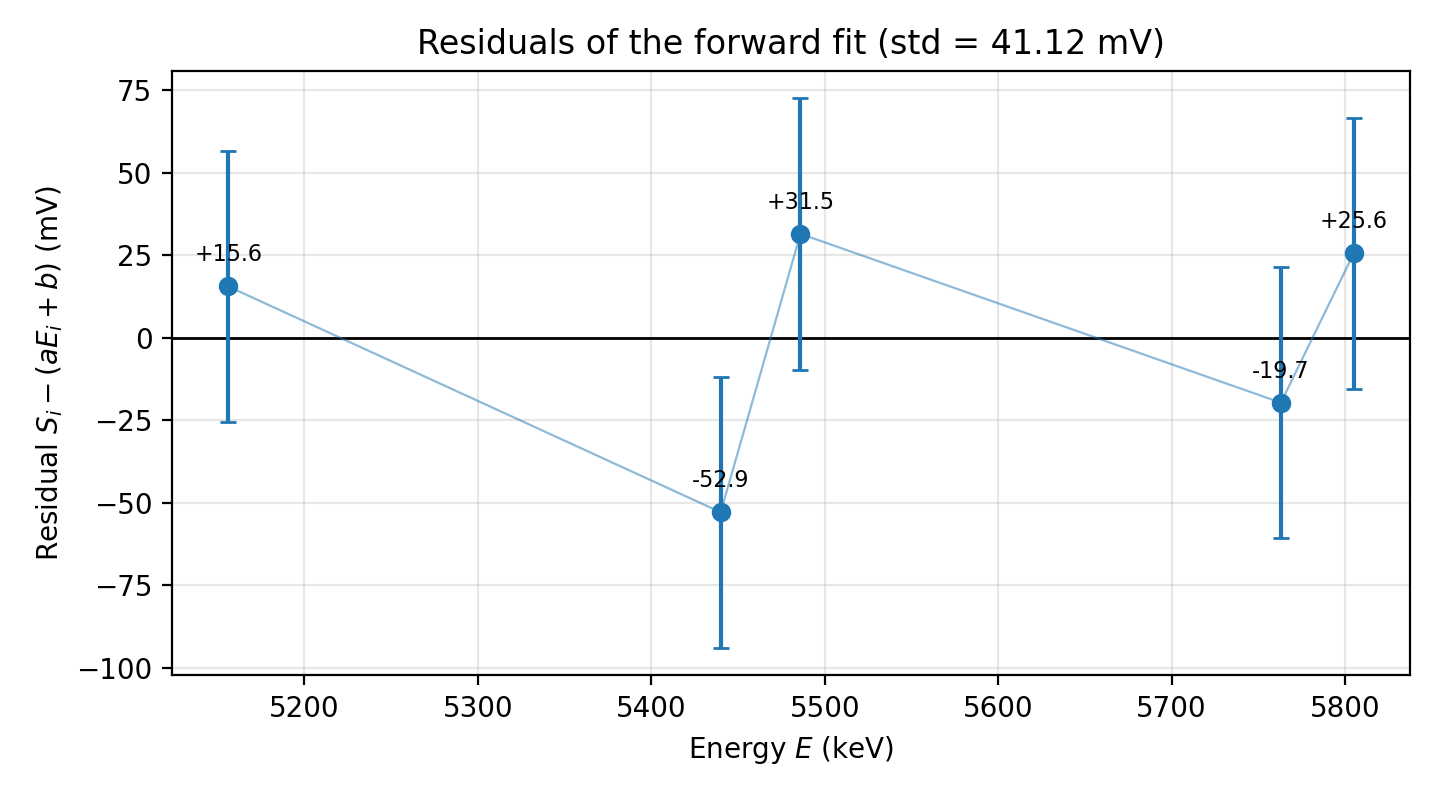
\includegraphics[width=0.74\textwidth]{hw2_residual.png}
  \caption{正向拟合的残差图。残差在零线两侧交错，无系统趋势。}
  \label{fig:resid}
\end{figure}

\subsection{物理意义}

\textbf{斜率与截距。}$a=0.4699$ mV/keV 即该探测系统的能量-幅度转换系数（灵敏度），其倒数 $1/a=2.128$ keV/mV 表示每毫伏信号约对应 $2.1$ keV 能量。截距 $b=-1048.6$ mV 是电子学零点偏移，本应过原点的直线因前放偏置等环节整体平移了。值得注意的是 $b$ 的标准误高达 $430$ mV（相对 $41\%$），远比 $a$ 的 $16.5\%$ 差：$E=0$ 距数据重心 $\bar E=5530$ keV 太远，由 5 个点外推到原点的截距自然约束得很差。好在本次反演并不需要用到远处的截距，所以这一点不影响结论；但若要把标定关系外推到很低能量，它就会成为主要误差来源。

\textbf{为什么可以用普通最小二乘。}$5156$、$5486$、$5805$ keV 分别与 $^{239}\mathrm{Pu}$、$^{241}\mathrm{Am}$、$^{244}\mathrm{Cm}$ 的主 $\alpha$ 线（$5.157$、$5.486$、$5.805$ MeV）吻合，提示标定源是一组标准 $\alpha$ 源（其余两个能量也应来自其他标准核素）。这些能量由核能级差决定、精度极高，因此可以放心地把 $E$ 当作无误差的自变量拟合 $S$，不必使用“两个变量都含误差”的更复杂方法。

\textbf{误差来源与量级。}$\sigma_{E_0}=97$ keV 中的主导项是 $s/|a|=87.5$ keV，也就是探测器自身的能量分辨：单个脉冲幅度就有 $41.12$ mV 的散布，相当于信号水平（$\bar S=1550$ mV）的 $2.65\%$，换算到能量即 $\pm87.5$ keV。标定曲线本身带来的不确定（约 $42.7$ keV）要小得多。这说明当前精度的主要限制不在标定，而在探测器分辨；若想提高精度，除了把标定做得更细（增加标定点、扩大能量跨度），更有效的是对同一粒子多测几个事件取平均。

\textbf{内插而非外推。}$S_0=1502$ mV 落在标定信号区间 $[1390,1705]$ mV 之内，对应能量 $5427$ keV 也落在 $[5156,5805]$ keV 之内。而且 $\bar S=1550.2$ mV，$S_0$ 与重心只差 $-48.2$ mV，误差公式里的杠杆项 $(S_0-\bar S)^2/(a^2S_{xx})$ 只有 $0.0376$，几乎可以忽略。这就是为什么 $E_0$ 的相对误差（$1.79\%$）远小于斜率本身的相对误差（$16.5\%$）：最小二乘直线绕重心转动，在重心附近做反演的误差最小。反之若未知粒子的幅度落在标定区间之外，杠杆项会迅速增大、误差成倍恶化——这正是标定工作总要留有余量、尽量让待测量落在标定区间内的原因。

\textbf{非线性的隐患。}$\alpha$ 粒子在闪烁体中会因电离密度高而发生\textbf{光产额淬灭}（如 Birks 定律描述的非线性：单位能量产生的光子数随 $\mathrm{d}E/\mathrm{d}x$ 增大而略减），原则上会使 $S(E)$ 在高能端轻微下弯。本题残差交错变号、没有系统趋势，说明在这段 $649$ keV 的窄窗口内这种弯曲小到被噪声掩盖，线性近似成立；但这属于“窗口内成立”的结论，不应外推到更宽的能量范围。

% =====================================================================
\section{AI使用说明}

本报告在撰写过程中使用人工智能工具（Claude Code + DeepSeek-4.1-Flash）辅助完成，具体用途如下：

\begin{enumerate}
  \item \textbf{撰写报告标题大纲。} 借助 AI 拟定报告的整体框架，在“题目解析—算法—结果讨论”的三节结构上细分，并梳理各节的标题与内容要点。
  \item \textbf{LaTeX 图文排版。} 借助 AI 完成 LaTeX 源文件的编写与排版，包括公式录入、结果图的插入与尺寸设置、表格绘制，以及页眉页脚、章节序号等版式调整。
  \item \textbf{物理结论检查。} 借助 AI 复核报告中的物理结论，包括最小二乘与逆回归公式的推导、不确定度的传递，并对关键数值作独立复算。
\end{enumerate}

以上即 AI 在本报告中的全部用途。

\end{document}
